\textbf{Ejemplo 3}\\

Una persona empieza el día primero de julio de 1986 a hacer depósitos de 1.000.000 COP
mensualmente el día primero de cada mes. Estos depósitos son efectuados en una entidad
financiera que le paga el 24\% nominal anual mes vencido; pero a partir del primero de
octubre de 1987 [15 períodos], decidió que de ahí en adelante sus depósitos serían de 2.500.000 COP
El último depósito lo hizo el primero de agosto de 1989. Si el primero de diciembre de 1989
decide cancelar la cuenta. ¿Cuál será el monto de sus ahorros?
\\

\textbf{Solución.}\\
%La tabla ira centrada
\begin{center}
	\renewcommand{\arraystretch}{1.5}% Margenes de las celdas
	%Creación de la cuadricula de 3 columnas
\begin{longtable}[H]{|c|c|c|}
		%Creamos una linea horizontal
\hline
		%Definimos el color de la primera fila
\rowcolor[HTML]{FFB183}
		%%%%% INICIO ASIGNACIÓN FECHA FOCAL %%%%%%%
		%%%%%%%%%% INICIO TITULO
		%Lo que se hace aquí es mezclar las 3 columnas en una sola
\multicolumn{3}{|c|}{\cellcolor[HTML]{FFB183}\textbf{1. Asignación período focal}}   \\ \hline
\multicolumn{3}{|c|} {$pf = 42 pmv$} \\ \hline
		%%%%%%%%%% FIN TITULO
  %%%%% INICIO DECLARACIÓN FORMULAS
  
%%%%%%%%%%% INICIO TITULO
\rowcolor[HTML]{FFB183}
\multicolumn{3}{|c|}{\cellcolor[HTML]{FFB183}\textbf{2. Declaración de variables}}    \\ \hline
%%%%%%%%%%% FIN TITULO
%%%%%%%%%%% INICIO MATEMÁTICAS

\multicolumn{2}{|c|}{$R_{1}$ = 1.000.000 COP }                       & $ n_{1} = 15 pmv $ \\ \hline
\multicolumn{2}{|c|}{$R_{3}$ = 2.500.000 COP $\hspace{0.3cm}$}       & $ n_{2} =27 pmv $ \\ \hline
\multicolumn{2}{|c|}{$j = 24\% namv \equiv 2\% pmv=i \hspace{0.3cm} $}	& $ n_{3} =23 pmv $ \\ \hline
\multicolumn{2}{|c|}{$VF = ? COP $}	                                & $ n_{4} = 4 pmv $ \\ \hline
%%%%%%%%%% FIN MATEMÁTICAS
		%%%%% INICIO FLUJO DE CAJA
\rowcolor[HTML]{FFB183}
\multicolumn{3}{|c|}{\cellcolor[HTML]{FFB183}\textbf{3. Diagrama de flujo de caja}} \\ \hline
		%Mezclamos 3 columnas y pondremos el dibujo
		%%%%%%%%%%%%% INSERCIÓN DE LA IMAGEN
		%Deberán descargar las imágenes respectivas del drive y pegarlas en la carpeta
		%n_capitulo/img/ejemplos/1/capitulo1ejemplo1.pdf  (el /1/ es el numero del ejemplo)
\multicolumn{3}{|c|}{ 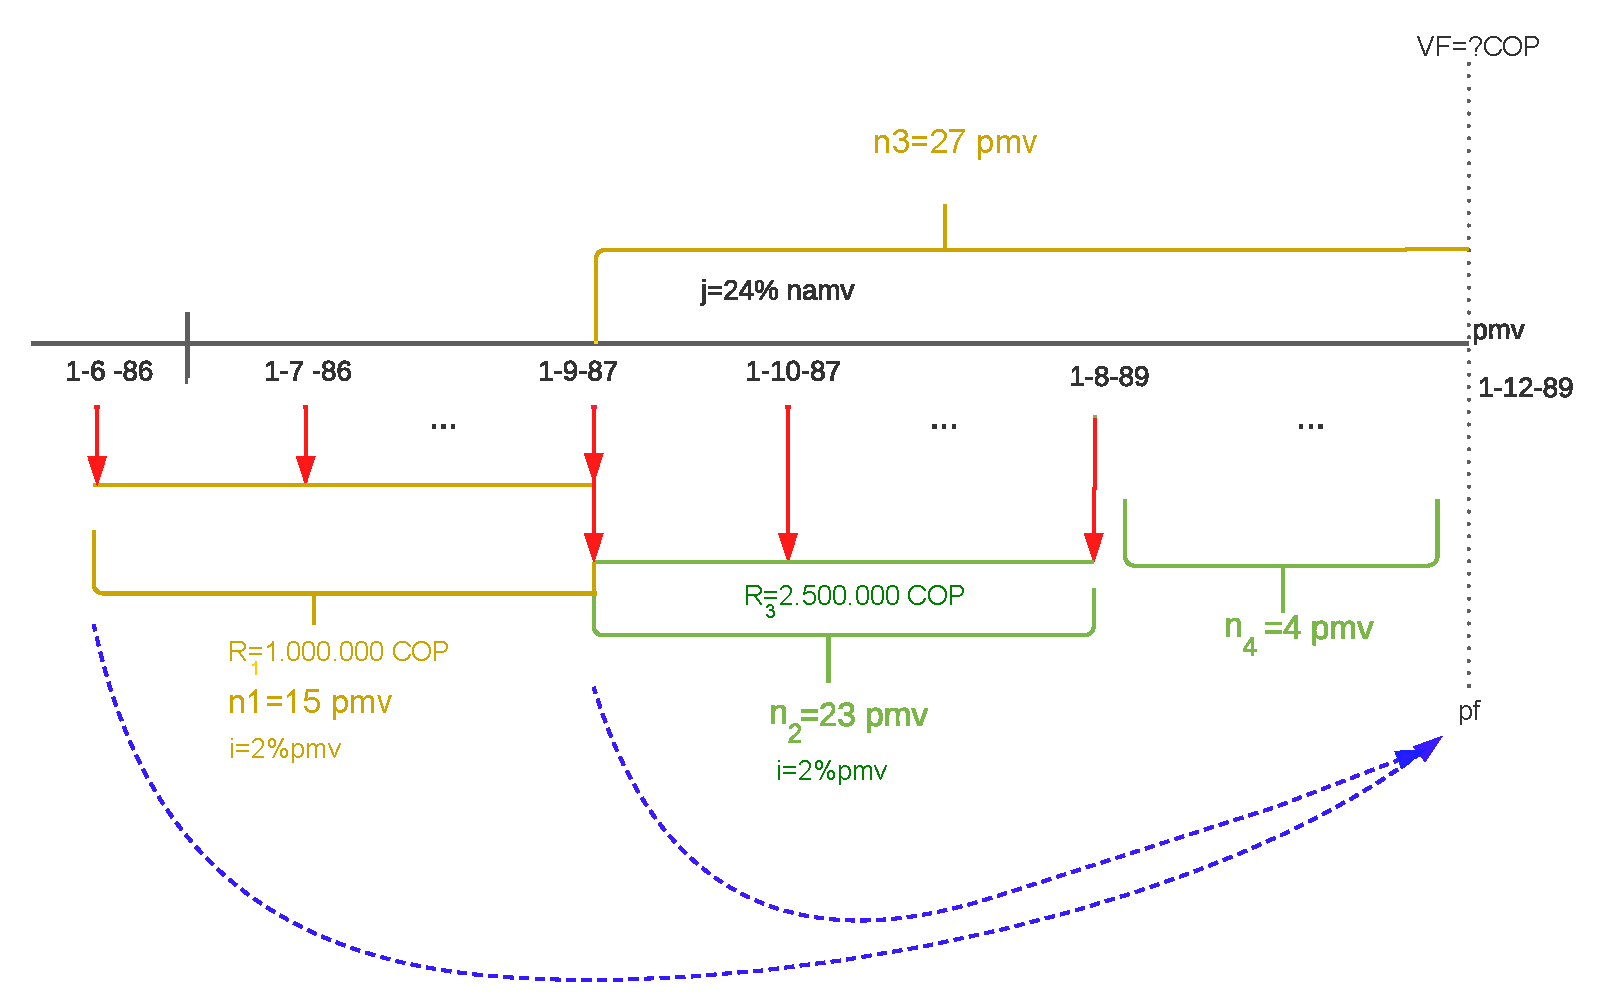
\includegraphics[scale=0.45, trim=-5 -5 -15 -30]{4_Capitulo/img/ejemplos/3/Capitulo4Ejercicio3.pdf} }   
   \\ \hline
		%%%%%%%%%%%%% FIN INSERCIÓN DE IMAGEN
		%%%%%FIN FLUJO DE CAJA
		
		
		
		%%%%% INICIO DECLARACIÓN FORMULAS
		%%%%%%%%%%% INICIO TITULO
\rowcolor[HTML]{FFB183}
\multicolumn{3}{|c|}{\cellcolor[HTML]{FFB183}\textbf{4. Declaración de fórmulas}}    \\ \hline
		%%%%%%%%%%% FIN TITULO
		%%%%%%%%%%% INICIO MATEMÁTICAS
\multicolumn{3}{|c|} {$VF=R\frac{(1+i)^{n}-1}{i}$ Valor futuro serie uniforme vencida}   \\ \hline	
	
		%%%%%%%%%% FIN MATEMÁTICAS
		%%%%%% INICIO DESARROLLO MATEMÁTICO
\rowcolor[HTML]{FFB183}
		%%%%%%%%%%INICIO TITULO
\multicolumn{3}{|c|}{\cellcolor[HTML]{FFB183}\textbf{5. Desarrollo matemático}}       \\ \hline
		%%%%%%%%%% FIN TITULO
		%%%%%%%%%% INICIO MATEMÁTICAS
\multicolumn{3}{|c|}		
{VF=1.000.000 COP $\frac{(1+0,02)^{15}-1}{0,02}\textcolor{Yellow}*[1+0.02]^{27} + 2.500.000 COP ^{\frac{(1+0.02)^{23}-1}{0.02}}\textcolor{Green}*[1+0.02]^{4}= $107.574.000,69 COP} \\
\multicolumn{3}{|c|}	
{VF = 107.574.001 COP}\\ \hline
		
		%%%%%%%%%% FIN MATEMÁTICAS
		%%%%%% FIN DESARROLLO MATEMÁTICO
		%%%%%% INICIO RESPUESTA
\rowcolor[HTML]{FFB183}
		%%%%%%%%%%INICIO TITULO
\multicolumn{3}{|c|}{\cellcolor[HTML]{FFB183}\textbf{6. Respuesta}}   \\ \hline
		%%%%%%%%%% FIN TITULO
		%%%%%%%%%% INICIO RESPUESTA MATEMÁTICA
\multicolumn{3}{|c|}{ El monto de sus ahorros será de 107.574.001 COP }  \\ \hline
		
		
		%%%%%%%%%% FIN MATEMÁTICAS
		%%%%%% FIN RESPUESTA
	\end{longtable}
	%Se crean dos lineas en blanco para que no quede el siguiente texto tan pegado
	%\newline \newline %USARLO SI CREES QUE ES NECESARIO
\end{center}
%%%%%%%%%%%%%%%%%%%%%%%%%%FIN EJERCICIO 3 %%%%%%%%%%%%%%%%%%%%%%%%%%%


\textbf{Tabla de rentabilidad en anual efectivo}\\
